\documentclass[11pt]{article}

\usepackage{geometry}
\geometry{margin=1in}
\usepackage{graphicx}
\usepackage[english]{babel}
\usepackage{fancyhdr}
\pagestyle{fancy}
\fancyhf{}
\lhead{Spring 2021 --- PHYS 432 Lab 5}
\rhead{Helen (Yeu) Chen}
\setlength{\parindent}{0cm}
\usepackage{makecell}
\usepackage{amsfonts}
\usepackage{longtable}
\usepackage{amsmath}
\usepackage{amssymb}
\usepackage{amsthm}
\usepackage{float}
\usepackage{caption}
\usepackage[outercaption]{sidecap}
\usepackage{multirow}
\graphicspath{ {./images/} }
\captionsetup[figure]{font=small,labelfont=small}


\fancyfoot[C]{\thepage}

\begin{document}
\textbf{Lamb Shift in Atomic Hydrogen Experiment}
\bigskip

\textbf{1. \textit{Introduction}}
\smallskip

In this experiment, we examined the fine structure and the Lamb shift of atomic hydrogen. Recall from the Zeeman effect experiment, an external B field applied on the electron's magnetic moment causes the energy level of electrons to split. A similar effect happens even without the present of an external B field. In short, the spin-orbit interaction adds an extra term in the Hamiltonian. It perturbs the original system and causes energy levels to split like in the Zeeman effect, this is what is known to be the fine structure (which also includes correction from relativistic energy). The splitted energy level of hydrogen could be described by (also called the Dirac result)
\begin{equation}\label{eqn:einstein}
E_{nj} = E_n [1+(\frac{\alpha}{n})^2 (\frac{n}{j+1/2} -\frac{3}{4})]
\end{equation}
where 
\begin{equation}\label{eqn:einstein}
E_n = - (\frac{\mu e^4}{(4 \pi \epsilon_0)^2 2\hbar})\frac{1}{n^2}
\end{equation}
and $\alpha$ is the fine structure constant defined by $\alpha = \frac{e^2}{4 \pi \epsilon_0\hbar c} \approx \frac{1}{137}$. As seen from eq. (1) and eq. (2), Dirac predict the energy level of hydrogen to be only depending on quantum number $n$ and $j$. However, Lamb and Retherford later discovered this not the case. They discovered that there is an energy difference between the lowest $n = 2$ states which are predicted to be degenerate by the Dirac theory. This phenomena is later known to be the Lamb shift. Even though people had suspicions on their findings at the time, their work led to the development of the quantum electrodynamics, an astonishing progress in the field of physics.

In our experiment, we looked at the spectrum from a hydrogen discharge lamp using the crossed-beam technique, in particular, the red region (i.e., the Balmer-alpha lines) of the spectrum corresponding to the following four transitions: $3D_{5/2} \rightarrow 2P_{3/2}$, $3P_{1/2} \rightarrow 2S_{1/2}$, $3P_{3/2} \rightarrow 2S_{1/2}$, and $3D_{3/2} \rightarrow 2P_{1/2}$. According to Dirac, the $3P_{3/2} \rightarrow 2S_{1/2}$ transition and the $3D_{3/2} \rightarrow 2P_{1/2}$ transition should have the same energy difference (since the both initial states have the same n, j values and so are the final states). However, we indeed observed that the $3D_{3/2} \rightarrow 2P_{1/2}$ spectral peak is position at a higher energy location than the $3P_{3/2} \rightarrow 2S_{1/2}$ spectral peak, indicating an evidence of the Lamb shift.
\bigskip

\textbf{2. \textit{The crossed-beam technique}}
\smallskip

In our experiment, we have used what is known as the crossed-beam technique to look at the atomic hydrogen spectrum, namely, the $n=2$ to $n=3$ transitions. This technique overcomes the difficulties arise from the Doppler shift. Recall from introductory physics, for a light source emitting light at a frequency $\nu_0$, let $\nu$ be the frequency an observer sees, then $\nu > \nu_0$ if the observer is moving towards the light source, and $\nu < \nu_0$ if the observer is moving away from the source. This is what is known as the Doppler effect.

For the atomic hydrogen we used in our experiment, all the atoms on average have a zero velocity. However, at a microscopic level the velocity distribution of the atoms actually follows a bell curve distribution centered at zero velocity. The range of velocities broadens the transition line, which obscures the fine structure. The crossed-beam technique uses two laser beams (one called pump beam or saturation beam and the other called probe beam), penetrating the atomic hydrogen discharge tube from the opposite directions as shown in Fig. 1. Notice that the beams are generated by splitting one laser source and are crossed in the tube. Also note that the probe beam is then sent to a detector for signal collection. 

Because the probe beam and the pump beam are moving in the opposite direction, for a moving atom, it sees that the probe beam and the pump beam have different laser frequencies. Let $\nu_0$ be the resonance frequency of the atom (i.e. a laser frequency that can cause excitation in the hydrogen atom in its rest frame) then if the laser frequency $\nu_{laser}$ is set to have $\nu_{laser} < \nu_0$, only atom moving towards left can interact with the probe beam, and if $\nu_{laser} > \nu_0$, then only atoms moving towards right can interact with the probe beam. The opposite is true for the pump beam. 

\begin{figure}[H]
\begin{center}
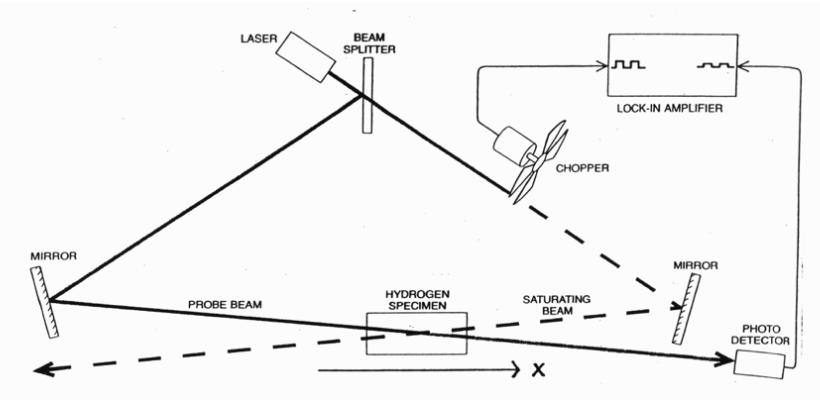
\includegraphics[width=10cm]{setup}
\label{Fig. 1}
\caption{Diagram showing the basic setup for the crossed-beam technique. The laser coming out from the tunable laser source splits into probe beam (solid line) and pump beam (dashed line, also called saturation beam) which travel through the discharge tube in opposite direction and is crossed inside the tube. The probe beam is then sent into a detector. The chopper and the lock-in amplifier helps reduce noise and strengthen targeted signals obtained from the detector.}
\end{center}
\end{figure}

\begin{figure}[H]
\begin{center}
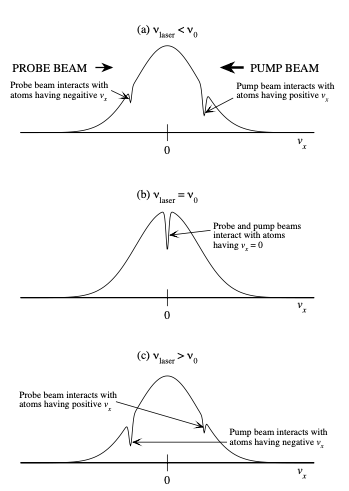
\includegraphics[width=6cm]{hole_burning}
\label{Fig. 2}
\caption{Velocity distribution curve showing the number of atoms that are available for absorption. (a) When $\nu_{laser} < \nu_0$, the probe interacts with atom moving left (defining positive direction to be right) and the opposite for the pump beam. (b) When $\nu_{laser} = \nu_0$, both beams interact with atoms at rest. (c) When $\nu_{laser} > \nu_0$, the probe interacts with atom moving right and the opposite for the pump beam.}
\end{center}
\end{figure}

When an atom interact with the laser beam, it is no longer available for another photon to cause the same excitation again, unless spontaneous emissions return the atom back to non-excited state. Fig. 2 shows the velocity distribution of the atoms and the dips represent when absorption of either pump beam or probe beam occurs. It shows that for $\nu_{laser} \ne \nu_0$, absorption of the probe beam and the pump beam occur on different subset of atoms, where one groups has positive velocity and the other group has negative velocity. Note that when $\nu_{laser} = \nu_0$ both beams interact with atoms at $v=0$. Since now both beams interact with the same set of atom, the detector watching the probe beam sees an increase in intensity because some atoms that used to absorb the probe beam at off resonance frequency now is absorbing the pump beam. Hence, the crossed-beam technique allows us to identify the resonance frequencies by watching for peaks in probe beam intensity. It overcomes the inconvenience that Doppler broadening brings us and in so doing allows a precise identification on closely spaced spectral peaks, enable us to better study the Lamb shift.
\bigskip

\textbf{3. \textit{Frequency shift measurement and final results}}
\smallskip

As seen from Fig. 1 the probe beam is sent to a detector for us to identify when the resonance occurs. However, there is one thing that is not included in the figure, that is, the pump beam is actually sent through the Fabry-Perot and the interferometry pattern is being observed by another detector, similar to the setup in the Zeeman effect experiment. The tunable laser source's wavelength is ramped across the four transition energy mentioned in section 1. With a fix Fabry-Perot mirror spacing, the spectral ring observed on the Fabry-Perot collapse to the center and causes the detector at the center to record a signal peak. The signals collected from both the Fabry-Perot and the probe beams is drawn simultaneously by the chart recorder. Since we know the Fabry-Perot peak spacing is what we called the free spectral range, which we can easily calculate ($FSR = c/2d$ where $d$ is the mirror spacing), the Fabry-Perot peaks location serves as a reference when calculating the frequency separations of the probe beam peaks. 

Using this technique, we have calculated the peaks separations for the following pairs of transitions: 
\begin{align*}
&2S_{1/2} - 3P_{3/2} \text{ to } 2P_{1/2} - 3D{3/2} \text{ (Lamb shift) }\\
&2P_{3/2} - 3D_{5/2} \text{ to } 2P_{1/2} - 3D{3/2}\\
&2P_{3/2} - 3D_{5/2} \text{ to } 2S_{1/2} - 3P{1/2}
\end{align*}

\begin{figure}[H]
\begin{center}
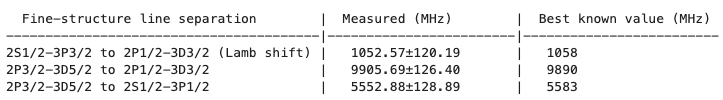
\includegraphics[width=14cm]{result}
\label{Fig. 3}
\caption{Table showing the measured and looked-up spectral peak separations (in MHz) among four different transition peaks in atomic hydrogen, namely: $3D_{5/2} \rightarrow 2P_{3/2}$, $3P_{1/2} \rightarrow 2S_{1/2}$, $3P_{3/2} \rightarrow 2S_{1/2}$, and $3D_{3/2} \rightarrow 2P_{1/2}$. The uncertainties is taken to be half of the FWHM of the spectral peaks we observed.}
\end{center}
\end{figure}

Fig. 3 summarize the measured peak separations in MHz and the looked-up best known values. As seen from the result, the measured values lies within $\pm30MHz$ of the best known values, definitely falls within the experimental uncertainties (which were taken to be half of the peak width of the probe beam peaks). This shows that our result agrees very well with the best known value.

 
\end{document}